% ============================================================
% Beamer — ISLP Lecture Series — IMPROVED EDITION
% Advanced Module A3: Conformal Prediction
% ============================================================
\documentclass[aspectratio=169,11pt]{beamer}
\usepackage[utf8]{inputenc}\usepackage[T1]{fontenc}\usepackage[english]{babel}
\usepackage{graphicx}\usepackage{booktabs}\usepackage{amsmath,amssymb,amsfonts}
\usepackage{mathtools}\usepackage{hyperref}\usepackage{xcolor}
\usepackage{verbatim}\usepackage{alltt}
\usepackage{tikz}\usetikzlibrary{calc,arrows.meta,positioning,shapes}
\usepackage{tcolorbox}\tcbuselibrary{skins}

\usetheme{Madrid}\usecolortheme{default}
\setbeamertemplate{navigation symbols}{}
\setbeamertemplate{footline}[frame number]
\setbeamertemplate{blocks}[rounded][shadow=false]
\setbeamertemplate{headline}{%
  \leavevmode\hbox{%
    \begin{beamercolorbox}[wd=\paperwidth,ht=2.2ex,dp=0.9ex]{section in head/foot}%
      {\fontsize{4.6}{5.2}\selectfont%
       \insertsectionnavigationhorizontal{\paperwidth}{}{\hskip0pt plus1filll}}%
    \end{beamercolorbox}}%
}
\setbeamerfont{section in head/foot}{size=\tiny}
\setbeamerfont{palette primary}{size=\tiny}
\setbeamerfont{palette tertiary}{size=\tiny}
\setbeamerfont{section in toc}{size=\footnotesize}

\usepackage{listings}
\definecolor{pyKw}{RGB}{0,0,180}\definecolor{pyStr}{RGB}{20,120,40}
\definecolor{pyCom}{RGB}{120,120,120}\definecolor{accent}{RGB}{38,70,140}
\lstdefinestyle{Pystyle}{language=Python,basicstyle=\ttfamily\footnotesize,
  keywordstyle=\color{pyKw}\bfseries,commentstyle=\color{pyCom}\itshape,
  stringstyle=\color{pyStr},showstringspaces=false,upquote=true,
  columns=fullflexible,breaklines=true,literate={~}{{$\sim$}}1}
\lstset{style=Pystyle}

% Tighter TOC spacing (place AFTER \lstset, BEFORE \AtBeginSection)
\usepackage{etoolbox}
\makeatletter
\patchcmd{\beamer@sectionintoc}{\vskip1.5em}{\vskip.6em}{\typeout{TOCPATCH-OK}}{\typeout{TOCPATCH-FAIL}}
\makeatother

\AtBeginSection[]{\begin{frame}{Outline}\footnotesize
  \tableofcontents[currentsection,sectionstyle=show/shaded,subsectionstyle=show/show/hide]
\end{frame}}

\newcommand{\islpsource}[1]{%
  \vfill\hfill{\tiny\itshape\color{gray}Source: #1 \textemdash{} ISLP, James et al.\ (2023).}\par
}

\newtcolorbox{takeaway}[1][Takeaway]{enhanced,colback=green!4,colframe=green!50!black,
  boxrule=0pt,leftrule=2.5pt,arc=2pt,fonttitle=\bfseries,title=#1,
  left=2mm,right=2mm,top=1mm,bottom=1mm}
\newtcolorbox{numexample}[1][Worked example]{enhanced,colback=orange!4,colframe=orange!70!black,
  boxrule=0pt,leftrule=2.5pt,arc=2pt,fonttitle=\bfseries,title=#1,
  left=2mm,right=2mm,top=1mm,bottom=1mm}
\newtcolorbox{readme}[1][How to read this]{enhanced,colback=blue!4,colframe=accent,
  boxrule=0pt,leftrule=2.5pt,arc=2pt,fonttitle=\bfseries,title=#1,
  left=2mm,right=2mm,top=1mm,bottom=1mm}

\title{Quantitative Research Methods}
\subtitle{Conformal Prediction\\[2pt]{\small Advanced module A3 --- optional self-study}}
\author{Prof.\ Dr.\ Christoph Weisser}
\date{}\graphicspath{{images/}}

\newtcolorbox{exercise}[1][Exercise]{enhanced, fontupper=\footnotesize, colback=purple!4, colframe=purple!55!black, boxrule=0pt, leftrule=2.5pt, arc=2pt, fonttitle=\bfseries, title=#1, left=2mm, right=2mm, top=1mm, bottom=1mm}
\newtcolorbox{solutionbox}[1][Solution]{enhanced, fontupper=\footnotesize, colback=teal!5, colframe=teal!55!black, boxrule=0pt, leftrule=2.5pt, arc=2pt, fonttitle=\bfseries, title=#1, left=2mm, right=2mm, top=1mm, bottom=1mm}
\newtcolorbox{longexercise}[1][Extended exercise (15 min)]{enhanced, fontupper=\footnotesize, colback=violet!6, colframe=violet!55!black, boxrule=0pt, leftrule=3pt, arc=2pt, fonttitle=\bfseries, title=#1, left=2mm, right=2mm, top=1mm, bottom=1mm}

% Reclaim ~2pt of body height (custom nav headline makes full slides tip over by ~1.83pt)
\addtobeamertemplate{frametitle}{}{\vspace{-2pt}}

\newtcolorbox{labnote}[1][Run this live in the lab notebook]{enhanced, fontupper=\footnotesize, colback=cyan!7, colframe=cyan!45!black, boxrule=0pt, leftrule=3pt, arc=2pt, fonttitle=\bfseries, title=#1, left=2mm, right=2mm, top=1mm, bottom=1mm}

% Industry application callout box --- slate grey, for real business/industry use
\definecolor{industryC}{RGB}{88,98,116}
\newtcolorbox{industry}[1][In industry]{enhanced, fontupper=\footnotesize, colback=industryC!7, colframe=industryC, boxrule=0pt, leftrule=3pt, arc=2pt, fonttitle=\bfseries, title={In industry --- #1}, left=2mm, right=2mm, top=1mm, bottom=1mm}

% Common-mistake callout --- crimson, for the error to pre-empt
\newtcolorbox{mistake}[1][Common mistake]{enhanced, fontupper=\footnotesize, colback=red!4, colframe=red!60!black, boxrule=0pt, leftrule=3pt, arc=2pt, fonttitle=\bfseries, title=#1, left=2mm, right=2mm, top=1mm, bottom=1mm}

\begin{document}
\begin{frame}[plain]\titlepage\end{frame}

\begin{frame}{Where this module fits}
  \footnotesize
  The four \textbf{advanced modules} are optional self-study decks that extend the
  twelve ISLP lectures. This one turns any predictive model from the course into a model
  with \emph{honest uncertainty}.
  \begin{center}
  \begin{tabular}{@{}p{4.6cm}p{8.6cm}@{}}
    \toprule
    \textbf{You already know (chapter)} & \textbf{What module A3 adds} \\
    \midrule
    Ch.\ 3 --- prediction intervals for linear regression &
      Intervals with \emph{guaranteed} coverage, without Gaussian errors or a correct
      model \\
    Ch.\ 5 --- train / validation splits &
      A third role for held-out data: the \emph{calibration set} \\
    Ch.\ 4 --- classifiers and their probabilities &
      Prediction \emph{sets}: ``\{flu, covid\}, with 90\% guarantee'' \\
    Ch.\ 8 --- gradient boosting &
      Boosted \emph{quantile} regression as the engine of adaptive intervals (CQR) \\
    \bottomrule
  \end{tabular}
  \end{center}
  \vspace{2pt}
  {\scriptsize Prerequisites: Chapters 3 and 5 are essential, Chapters 4 and 8 helpful.
  Short exercises every $\sim$20 min; extended exercises every $\sim$45 min; the module
  has a companion lab notebook.}
\end{frame}

\begin{frame}{Contents}\small\tableofcontents[hideallsubsections]
  \vfill
  {\tiny Optional and advanced material is collected in the \textbf{appendix} at the end of the deck.}
\end{frame}

\begin{frame}{Notation in this module}
  \footnotesize
  \begin{center}
  \begin{tabular}{@{}ll@{}}
    \toprule
    \textbf{Symbol} & \textbf{Meaning} \\
    \midrule
    $(x_i, y_i)$ & feature--response pair of observation $i$ \\
    $\mathcal{D}_{\text{tr}}$, $\mathcal{D}_{\text{cal}}$ & proper training set and calibration set (disjoint) \\
    $n$ & number of calibration points, $n = |\mathcal{D}_{\text{cal}}|$ \\
    $\hat f$ & prediction rule fitted on $\mathcal{D}_{\text{tr}}$ only \\
    $s_i$ & conformity score of calibration point $i$ (e.g.\ $|y_i - \hat f(x_i)|$) \\
    $s_{(k)}$ & $k$-th smallest calibration score (order statistic) \\
    $\alpha$ & target miscoverage level (we use $\alpha = 0.1$: 90\% coverage) \\
    $\hat q$ & conformal quantile: $s_{(k)}$ with $k = \lceil (n+1)(1-\alpha) \rceil$ \\
    $C(x)$ & prediction interval (regression) or prediction set (classification) \\
    $\rho_\tau(u)$ & pinball loss of quantile regression at level $\tau$ \\
    $\hat q_{\text{lo}}, \hat q_{\text{hi}}$ & fitted conditional quantile curves (levels $\alpha/2$, $1-\alpha/2$) \\
    $\hat p_k(x)$ & estimated probability of class $k$ at $x$ (softmax output) \\
    $K$ & number of classes \\
    \bottomrule
  \end{tabular}
  \end{center}
\end{frame}

\begin{frame}{Sources and references}
  \begin{block}{Primary textbook}
    James, G., Witten, D., Hastie, T., Tibshirani, R., \& Taylor, J.\ (2023).
    \emph{An Introduction to Statistical Learning, with Applications in
    Python.} Springer. (Chapters 3 and 5 supply the prerequisites.)
  \end{block}
  \begin{block}{Further reading on conformal prediction}
    \footnotesize
    Vovk, V., Gammerman, A., \& Shafer, G.\ (2005). \emph{Algorithmic Learning in a
    Random World.} Springer. ---
    Lei, J., et al.\ (2018). Distribution-free predictive inference for regression.
    \emph{JASA} 113(523). ---
    Romano, Y., Patterson, E., \& Cand\`es, E.\ (2019). Conformalized quantile
    regression. \emph{NeurIPS}. ---
    Angelopoulos, A., \& Bates, S.\ (2023). Conformal prediction: a gentle introduction.
    \emph{Foundations and Trends in Machine Learning} 16(4).
  \end{block}
\end{frame}

\begin{frame}{Learning objectives}
  By the end of this module you will be able to:
  \begin{itemize}
    \item \textbf{Explain} why classical prediction intervals need assumptions that
          conformal prediction drops.
    \item \textbf{State} exchangeability and \textbf{judge} when it is plausible.
    \item \textbf{Apply} split conformal prediction: compute $\hat q$ and the interval
          by hand and in Python.
    \item \textbf{Distinguish} marginal from conditional coverage --- and say which one
          is guaranteed.
    \item \textbf{Build} adaptive intervals with conformalized quantile regression (CQR).
    \item \textbf{Construct} prediction sets for classifiers and read their sizes.
    \item \textbf{Avoid} the pitfalls: leakage into the calibration set, time series,
          tiny calibration sets.
  \end{itemize}
\end{frame}

\begin{frame}{Roadmap of this module}
  \begin{takeaway}[Uncertainty you can guarantee]
    \begin{enumerate}
      \item Why a point prediction is a guess --- and what Ch.\ 3's intervals assume.
      \item Exchangeability: the one assumption conformal prediction needs.
      \item Split conformal for regression: the whole recipe, and its proof sketch.
      \item Marginal vs conditional coverage --- the honest reading of the guarantee.
      \item Adaptive intervals: locally weighted scores and CQR.
      \item Prediction sets for classification; conformal vs the classical interval;
            pitfalls and production practice.
    \end{enumerate}
  \end{takeaway}
\end{frame}

\begin{frame}{Where conformal prediction is used in industry}
  \scriptsize
  \begin{center}
  \begin{tabular}{@{}p{2.6cm}p{5.2cm}p{4.6cm}@{}}
    \toprule
    \textbf{Sector} & \textbf{Concrete application} & \textbf{Which decision it drives} \\
    \midrule
    Energy & Intervals around day-ahead load and wind forecasts & How much reserve
      capacity to buy \\
    E-commerce, logistics & Delivery-time windows behind the checkout promise &
      Which arrival dates to display and guarantee \\
    Healthcare & Prediction sets over diagnoses in triage support & Which cases are
      routed to a human specialist \\
    Banking & Intervals on loss and prepayment forecasts & Capital buffers; which cases
      go to manual review \\
    Pharma R\&D & Conformal sets in virtual screening of compounds & Which molecules
      advance to the wet lab \\
    Manufacturing & Set-valued defect classification on the line & Which parts get
      pulled for manual inspection \\
    \bottomrule
  \end{tabular}
  \end{center}
  \begin{industry}[The common thread]
    In every row the model's \emph{point} prediction was already available --- the money
    is in the \textbf{width of the interval} or the \textbf{size of the set}, because
    that is what sizes the buffer, the promise, or the manual-review queue.
  \end{industry}
\end{frame}

\begin{frame}{Industry case in depth: the delivery promise at an online retailer}
  \footnotesize
  \begin{industry}[The problem: a point ETA is a promise you will break]
    The checkout page must commit to an arrival date. A gradient-boosted model predicts
    delivery time from warehouse, carrier, destination and weekday --- but showing its
    point estimate (``arrives Wednesday'') is wrong for a large share of parcels, and
    every miss costs a support ticket or a refund. What the business needs is a
    \textbf{window} (``Tuesday--Thursday'') that holds, say, 90\% of the time.
  \end{industry}
  \begin{readme}[How conformal prediction is wired in]
    Last month's delivered parcels are split: most \textbf{retrain} the model, a held-out
    slice becomes the \textbf{calibration set}. Absolute errors on that slice give
    $\hat q$; the site displays $\hat f(x) \pm \hat q$ rounded to days. Recalibration
    runs \emph{weekly}, so carrier disruptions feed into $\hat q$ within days; a
    dashboard tracks realised coverage and median window width.
  \end{readme}
  \begin{takeaway}[Two honest caveats]
    Delivery times \emph{drift} (peak season, strikes) --- exchangeability between
    calibration and next week is an approximation, hence the weekly recalibration.
    And the guarantee is \emph{marginal}: remote postcodes can be undercovered while
    city centres are overcovered, unless calibration is done per group.
  \end{takeaway}
\end{frame}

% ============================================================
\section{Why Conformal}
% ============================================================

\begin{frame}{A point prediction without uncertainty is a guess}
  Take the \texttt{Wage} data ($n = 3\,000$ workers): predict \textbf{wage} from
  \textbf{age}.
  \begin{numexample}[How much do 45-year-olds actually earn?]
    Among the 268 workers aged 44--46, wages average \$$120\,400$ --- but they range
    from \$$36\,700$ to \$$318\,300$, with a standard deviation of \$$43\,400$.
    A model that answers ``\$120k'' communicates \emph{none} of that spread: the single
    number is a guess dressed up as knowledge.
  \end{numexample}
  \begin{itemize}
    \item Every model from this course --- linear regression, boosting, a neural net ---
          produces $\hat f(x)$. The question this module answers: \emph{how far can the
          truth be from $\hat f(x)$, with a guarantee?}
    \item We want a recipe that works for \textbf{any} $\hat f$, on \textbf{finite}
          samples, \textbf{without} trusting the model.
  \end{itemize}
  \begin{industry}[Pricing and planning: the interval is the product]
    A buyer sizing stock, a hospital planning beds, a grid operator buying reserve ---
    none of them can act on ``the forecast is 120''. They act on ``between 80 and 160,
    9 times out of 10''.
  \end{industry}
\end{frame}

\begin{frame}{What Chapter 3 gave us --- and what it silently assumed}
  \footnotesize
  \begin{block}{The classical 90\% prediction interval (Ch.\ 3)}
    Under the linear model $Y = X\beta + \varepsilon$ with
    $\varepsilon \sim \mathcal{N}(0, \sigma^2)$ i.i.d.:
    \quad $\hat y_0 \;\pm\; t_{n-p-1,\,0.95}\;\hat\sigma
      \sqrt{1 + x_0^\top (X^\top X)^{-1} x_0}$.
  \end{block}
  \begin{readme}[The fine print --- three assumptions doing all the work]
    \begin{enumerate}
      \item \textbf{Correct mean model}: $E[Y \mid X = x]$ really is linear in $x$.
      \item \textbf{Gaussian errors}: the $t$/normal quantile calibrates the width.
      \item \textbf{Homoskedasticity}: one $\sigma$ for every $x$.
    \end{enumerate}
    Break any of the three and the ``90\%'' printed by \texttt{statsmodels} is a claim,
    not a fact.
  \end{readme}
  \begin{numexample}[Wage breaks the fine print]
    Wages are strongly right-skewed (skewness $1.68$; 79 workers, $2.6\%$, earn above
    \$250k). The Gaussian recipe $\hat f(x) \pm 1.645\,\hat\sigma$ gives half-width
    $66.1$ --- and covers $95.2\%$ of test wages while \emph{claiming} 90\%:
    miscalibrated and needlessly wide.
  \end{numexample}
\end{frame}

\begin{frame}{The conformal promise}
  \begin{block}{What conformal prediction guarantees}
    From any fitted model $\hat f$ and a calibration set of $n$ held-out points, build
    $C(x)$ such that for a new exchangeable point $(X_{n+1}, Y_{n+1})$:
    \[
      \boxed{\;\Pr\big(Y_{n+1} \in C(X_{n+1})\big) \;\ge\; 1 - \alpha\;}
    \]
  \end{block}
  \footnotesize
  \begin{readme}[Why this is remarkable --- read the guarantee word by word]
    \begin{itemize}
      \item \textbf{Distribution-free}: no Gaussian errors, no model for
            $P(Y \mid X)$ --- wages can be as skewed as they like.
      \item \textbf{Finite-sample}: holds exactly at $n = 500$, not just as
            $n \to \infty$.
      \item \textbf{Any model}: $\hat f$ may be misspecified, overfit, or a black box.
      \item \textbf{Marginal}: averaged over the new point \emph{and} the calibration
            draw --- more on this honest word soon.
    \end{itemize}
  \end{readme}
  \begin{takeaway}
    Conformal trades ``if my model is right, coverage is exact at every $x$'' for
    ``\emph{whatever} my model is, coverage is right \emph{on average}''.
  \end{takeaway}
\end{frame}

% ------------------------------------------------------------
\begin{frame}{Exercise A3.1 --- What did we just buy? [Concept]}
\begin{exercise}
  \begin{enumerate}
    \item Name the three assumptions behind the Chapter 3 prediction interval.
    \item Which of the three does conformal prediction keep, and what does it demand
          instead?
    \item A colleague says: ``With conformal prediction, my 90\% interval covers the
          true wage of \emph{every 45-year-old} with probability 90\%.'' Is that what
          the guarantee says?
    \item Why does an overfit $\hat f$ not break the conformal guarantee (hint: where
          are the residuals computed)?
  \end{enumerate}
\end{exercise}
\end{frame}

\begin{frame}{Solution --- Exercise A3.1}
\begin{solutionbox}
  \textbf{Method.} Compare the two guarantees assumption by assumption.
  \begin{itemize}
    \item \textbf{Part 1.} Correct (linear) mean model; Gaussian errors;
          homoskedastic errors (one $\sigma$ for all $x$).
    \item \textbf{Part 2.} It keeps \emph{none} of them. Instead it demands
          (i) \textbf{exchangeability} between calibration and test points and
          (ii) a \textbf{clean split}: $\hat f$ never sees the calibration data.
    \item \textbf{Part 3.} No. The guarantee is \textbf{marginal}: averaged over all
          new points (and calibration draws), at least 90\% are covered. Coverage
          \emph{among 45-year-olds specifically} may be higher or lower --- we will
          measure exactly this on Wage ($98.6\%$ for under-30s, $82.9\%$ for
          60-plus, same interval).
    \item \textbf{Part 4.} The scores are residuals on \emph{held-out} calibration
          points. An overfit $\hat f$ produces \emph{large} held-out residuals, so
          $\hat q$ grows and the interval honestly widens --- the guarantee survives;
          only the width suffers.
  \end{itemize}
\end{solutionbox}
\begin{mistake}
  Reading ``90\%'' as a per-person (conditional) probability. Marginal coverage is a
  statement about the \emph{average} over the population, not about your specific $x$.
\end{mistake}
\end{frame}

% ============================================================
\section{Split Conformal}
% ============================================================

\begin{frame}{Exchangeability --- the one assumption we need}
  \footnotesize
  \begin{block}{Definition}
    Random variables $Z_1, \dots, Z_m$ are \textbf{exchangeable} if for every
    permutation $\pi$,
    \[
      (Z_{\pi(1)}, \dots, Z_{\pi(m)}) \overset{d}{=} (Z_1, \dots, Z_m).
    \]
  \end{block}
  \begin{readme}[What it means in plain words]
    \begin{itemize}
      \item Every \emph{ordering} of the data is equally likely --- the labels
            ``calibration point 17'' and ``test point'' carry no information.
      \item \textbf{i.i.d.\ $\Rightarrow$ exchangeable}, but not conversely:
            exchangeability is \emph{weaker} (e.g.\ sampling without replacement).
      \item Key consequence: among $n + 1$ exchangeable scores with no ties, the
            \textbf{rank} of the last one is \emph{uniform} on $\{1, \dots, n+1\}$.
    \end{itemize}
  \end{readme}
  \begin{takeaway}
    Conformal prediction is rank arithmetic on exchangeable scores. Everything follows
    from ``the new point is nothing special''.
  \end{takeaway}
\end{frame}

\begin{frame}{The honest slide: what breaks exchangeability}
  \footnotesize
  \begin{itemize}
    \item \textbf{Time series}: today's demand depends on yesterday's --- orderings
          are \emph{not} equally likely, and tomorrow may differ systematically.
    \item \textbf{Covariate shift}: calibrate on last year's customers, deploy on a
          new market --- the $X$-distribution moved.
    \item \textbf{Feedback loops}: the model's own decisions (credit granted, price
          shown) change the data it will be judged on.
  \end{itemize}
  \begin{readme}[What still works]
    Violations degrade the guarantee \emph{gradually}, and there are repairs:
    \emph{weighted} conformal under known covariate shift (Tibshirani et al., 2019),
    blocked or online variants for dependence. This module sticks to the exchangeable
    case --- the pitfalls section returns here.
  \end{readme}
  \begin{industry}[Model monitoring: coverage as an alarm]
    Production ML teams track \emph{realised coverage} weekly. Coverage sliding from
    90\% to 80\% is a drift detector that needs no labels beyond the ones you already
    collect --- often the first sign that the world has moved away from the training
    distribution.
  \end{industry}
\end{frame}

\begin{frame}{Split conformal --- the pipeline (native diagram)}
  \begin{center}
  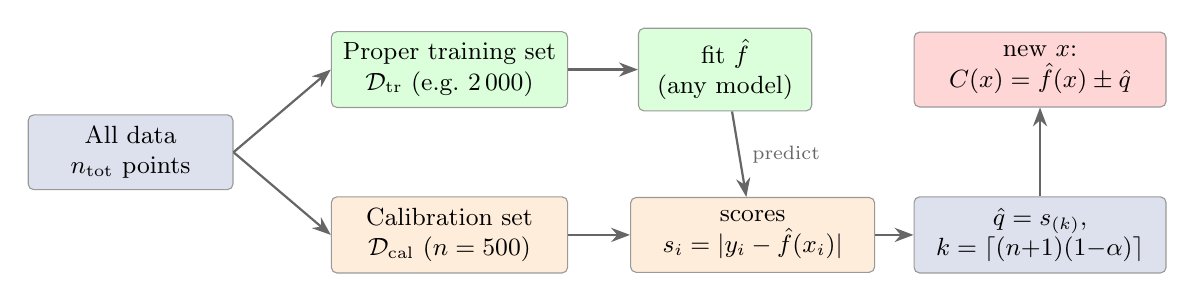
\begin{tikzpicture}[font=\small,
      box/.style={draw=black!40, rounded corners=2pt, align=center,
                  minimum height=0.95cm, inner sep=4pt},
      arr/.style={-{Stealth[length=2.4mm]}, thick, black!60}]
    \node[box, fill=accent!16, minimum width=2.6cm] (data) at (0, 0) {All data\\$n_{\text{tot}}$ points};
    \node[box, fill=green!14, minimum width=3.0cm] (train) at (4.05, 1.05) {Proper training set\\$\mathcal{D}_{\text{tr}}$ (e.g.\ $2\,000$)};
    \node[box, fill=orange!14, minimum width=3.0cm] (cal) at (4.05, -1.05) {Calibration set\\$\mathcal{D}_{\text{cal}}$ ($n = 500$)};
    \node[box, fill=green!14, minimum width=2.2cm] (fit) at (7.55, 1.05) {fit $\hat f$\\(any model)};
    \node[box, fill=orange!14, minimum width=3.1cm] (scores) at (7.9, -1.05) {scores\\$s_i = |y_i - \hat f(x_i)|$};
    \node[box, fill=accent!16, minimum width=3.2cm] (qhat) at (11.55, -1.05) {$\hat q = s_{(k)}$,\\$k = \lceil (n{+}1)(1{-}\alpha) \rceil$};
    \node[box, fill=red!16, minimum width=3.2cm] (pred) at (11.55, 1.05) {new $x$:\\$C(x) = \hat f(x) \pm \hat q$};
    \draw[arr] (data.east) -- (train.west);
    \draw[arr] (data.east) -- (cal.west);
    \draw[arr] (train) -- (fit);
    \draw[arr] (cal) -- (scores);
    \draw[arr] (fit) -- node[right=1pt, font=\scriptsize]{predict} (scores);
    \draw[arr] (scores) -- (qhat);
    \draw[arr] (qhat) -- (pred);
  \end{tikzpicture}
  \end{center}
  \begin{takeaway}
    One split, one model fit, one sorted list of residuals, one quantile. The model
    only ever sees $\mathcal{D}_{\text{tr}}$; the guarantee only ever uses
    $\mathcal{D}_{\text{cal}}$.
  \end{takeaway}
\end{frame}

\begin{frame}{The whole recipe on one slide}
  \begin{block}{Algorithm: split conformal prediction for regression}
    \begin{enumerate}
      \item Split the data into $\mathcal{D}_{\text{tr}}$ and
            $\mathcal{D}_{\text{cal}}$ (sizes e.g.\ $2\,000$ and $n = 500$).
      \item Fit $\hat f$ on $\mathcal{D}_{\text{tr}}$ \emph{only}.
      \item Compute calibration scores $s_i = |y_i - \hat f(x_i)|$ for
            $i \in \mathcal{D}_{\text{cal}}$.
      \item Set
            $\;\boxed{\;\hat q = s_{(k)}, \qquad k = \big\lceil (n+1)(1-\alpha) \big\rceil\;}$
            \; --- the $k$-th smallest score.
      \item For any new $x$ report
            $\;C(x) = \big[\hat f(x) - \hat q,\; \hat f(x) + \hat q\big]$.
    \end{enumerate}
  \end{block}
  \begin{readme}[Decoding the boxed formula]
    $n$ = number of calibration points; $\alpha$ = tolerated miscoverage
    ($0.1$ for a 90\% interval); $s_{(k)}$ = the $k$-th order statistic of the sorted
    scores; the ceiling $\lceil \cdot \rceil$ rounds \emph{up}, so $\hat q$ is the
    $\tfrac{k}{n}$ empirical quantile --- slightly \emph{above} the naive
    $(1-\alpha)$-quantile. With $n = 500$, $\alpha = 0.1$:
    $k = \lceil 501 \times 0.9 \rceil = 451$, the $0.902$ quantile.
  \end{readme}
\end{frame}

\begin{frame}{Why the odd index? A tiny worked example}
  \footnotesize
  \begin{numexample}[Nine calibration scores at 10\% miscoverage]
    Scores: $1.2,\; 0.4,\; 2.8,\; 0.9,\; 1.7,\; 3.5,\; 0.6,\; 2.1,\; 1.0$.
    Sorted: $0.4,\ 0.6,\ 0.9,\ 1.0,\ 1.2,\ 1.7,\ 2.1,\ 2.8,\ 3.5$. Then
    $k = \lceil (9+1)(0.9) \rceil = 9 \Longrightarrow \hat q = s_{(9)} = 3.5$
    (the maximum!). At $\alpha = 0.2$: $k = \lceil 10 \times 0.8 \rceil = 8$, so
    $\hat q = s_{(8)} = 2.8$. At $n = 19$, $\alpha = 0.1$:
    $k = \lceil 20 \times 0.9 \rceil = 18$ --- the 18th of 19.
  \end{numexample}
  \begin{readme}[The intuition for the ``$+1$'']
    The new point's score joins the $n$ calibration scores as an $(n{+}1)$-th,
    equally-ranked member. To catch it with probability $\ge 0.9$ we must clear at
    least $90\%$ of \emph{all $n+1$ ranks} --- hence $(n+1)(1-\alpha)$, rounded up
    because ranks are integers. The naive $90\%$ quantile of $n$ scores would
    undercover, worst at small $n$.
  \end{readme}
  \begin{takeaway}
    Small calibration sets force conservative quantiles: with $n = 9$ the 90\%
    interval must stretch to the \emph{largest} observed residual.
  \end{takeaway}
\end{frame}

\begin{frame}{The coverage guarantee, and why it is true}
  \footnotesize
  \begin{block}{Theorem (split conformal coverage)}
    If the calibration pairs and the test pair are exchangeable, and $\hat f$ was fit
    without touching them, then
    \[
      1 - \alpha \;\le\; \Pr\big(Y_{n+1} \in C(X_{n+1})\big)
      \;\le\; 1 - \alpha + \tfrac{1}{n+1},
    \]
    the upper bound requiring almost-surely distinct scores.
  \end{block}
  \begin{readme}[Proof sketch --- three lines of rank arithmetic]
    \begin{enumerate}
      \item Let $s_{n+1} = |Y_{n+1} - \hat f(X_{n+1})|$ join the $n$ calibration
            scores. All $n+1$ scores are exchangeable (each is the same function of its
            own data point, with $\hat f$ fixed).
      \item Coverage happens $\iff s_{n+1} \le s_{(k)} \iff$
            $\operatorname{rank}(s_{n+1}) \le k$ among the $n+1$ scores.
      \item That rank is uniform on $\{1, \dots, n+1\}$, so coverage
            $= \tfrac{k}{n+1} \ge \tfrac{(n+1)(1-\alpha)}{n+1} = 1 - \alpha$.
            \hfill (Full argument: appendix.)
    \end{enumerate}
  \end{readme}
  \begin{numexample}[How tight is the guarantee at $n$ of 500?]
    $k = 451 \Rightarrow$ coverage is pinned between $0.9$ and
    $0.9 + \tfrac{1}{501} = 0.902$ --- not just a bound, essentially an
    \emph{equality}.
  \end{numexample}
\end{frame}

\begin{frame}{Wage: the calibration quantile and the band it buys}
  \begin{center}
    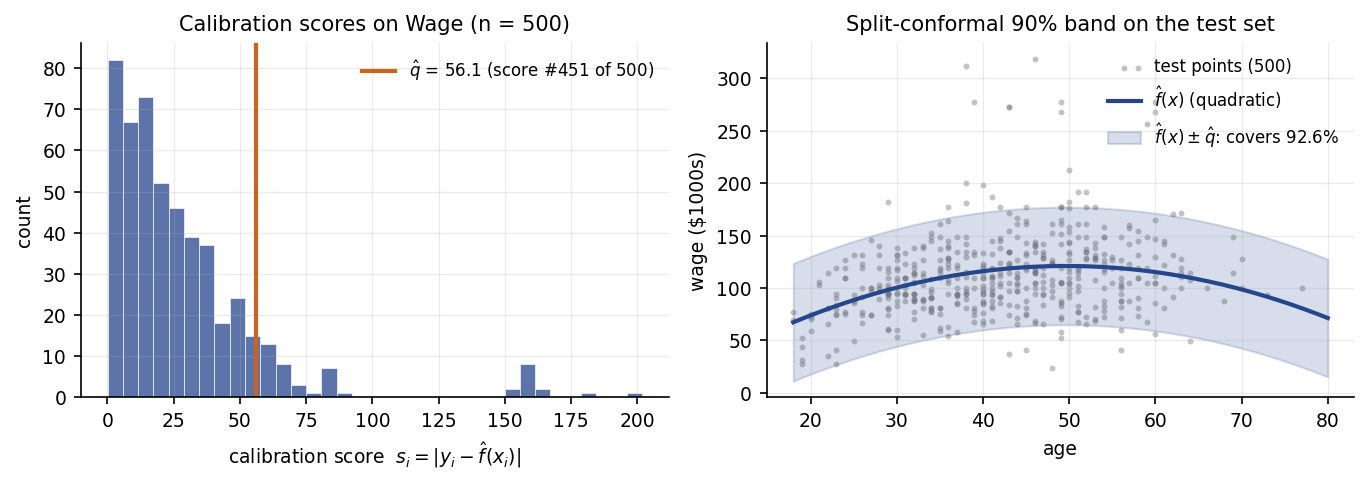
\includegraphics[width=0.92\textwidth,height=0.55\textheight,keepaspectratio]{a3_scores_band.png}
  \end{center}
  \begin{takeaway}
    Quadratic fit on $2\,000$ training points; the $451$st of $500$ sorted calibration
    residuals gives $\hat q = 56.1$. The band $\hat f(\text{age}) \pm 56.1$ covers
    $92.6\%$ of the 500 test wages --- and is \emph{narrower} than the miscalibrated
    Gaussian band ($\pm 66.1$, covering $95.2\%$).
  \end{takeaway}
  \begin{labnote}[Notebook \S1: split conformal on Wage]
    \texttt{advanced\_03\_conformal\_lab.ipynb}, \S1 builds exactly this: the split
    (seed 2024), the sorted scores, $\hat q = 56.14$ and the test coverage $0.926$ ---
    about ten lines of numpy.
  \end{labnote}
\end{frame}

% ------------------------------------------------------------
\begin{frame}{Exercise A3.2 --- Computing the conformal quantile by hand [Math]}
\begin{exercise}
  A model is calibrated on $n = 9$ held-out points with absolute residuals
  \[
    2.1,\quad 0.7,\quad 4.0,\quad 1.3,\quad 0.5,\quad 2.9,\quad 1.8,\quad 5.2,\quad 1.1 .
  \]
  \begin{enumerate}
    \item Compute $\hat q$ for $\alpha = 0.2$ and write down $C(x)$ if
          $\hat f(x) = 100$.
    \item Compute $\hat q$ for $\alpha = 0.1$. What do you notice?
    \item For $n = 99$ and $\alpha = 0.05$: which order statistic is $\hat q$?
    \item Exactly which coverage does the theorem guarantee in part 3
          (both bounds)?
  \end{enumerate}
\end{exercise}
\end{frame}

\begin{frame}{Solution --- Exercise A3.2}
\begin{solutionbox}
  \textbf{Method.} Sort, compute $k = \lceil (n+1)(1-\alpha) \rceil$, pick $s_{(k)}$.
  Sorted scores: $0.5,\ 0.7,\ 1.1,\ 1.3,\ 1.8,\ 2.1,\ 2.9,\ 4.0,\ 5.2$.
  \begin{itemize}
    \item \textbf{Part 1.} $k = \lceil 10 \times 0.8 \rceil = 8 \Rightarrow
          \hat q = s_{(8)} = 4.0$, so $C(x) = [96.0,\ 104.0]$.
    \item \textbf{Part 2.} $k = \lceil 10 \times 0.9 \rceil = 9 \Rightarrow
          \hat q = s_{(9)} = 5.2$ --- the \emph{maximum}. With only 9 calibration
          points, a 90\% guarantee forces the most conservative choice available.
    \item \textbf{Part 3.} $k = \lceil 100 \times 0.95 \rceil = 95 \Rightarrow$
          $\hat q$ is the \textbf{95th smallest of 99} scores.
    \item \textbf{Part 4.} Coverage lies in
          $\big[\tfrac{95}{100},\ \tfrac{95}{100} + \tfrac{1}{100}\big] = [0.95,\ 0.96]$
          --- read off as $k/(n+1) = 95/100$ and $k/(n+1) + 1/(n+1)$.
  \end{itemize}
  \textbf{Take-away.} $\hat q$ is always a \emph{single order statistic} --- no
  interpolation, no model, just a sorted list and one index.
\end{solutionbox}
\begin{mistake}
  Computing the plain $90\%$ empirical quantile ($0.9 \times 9 = 8.1$, so interpolating
  near $s_{(8)}$). The conformal index uses $n + 1$, not $n$ --- forgetting the $+1$
  is precisely what loses the finite-sample guarantee.
\end{mistake}
\end{frame}

\begin{frame}{The guarantee is an average over splits --- see it hold}
  \begin{center}
    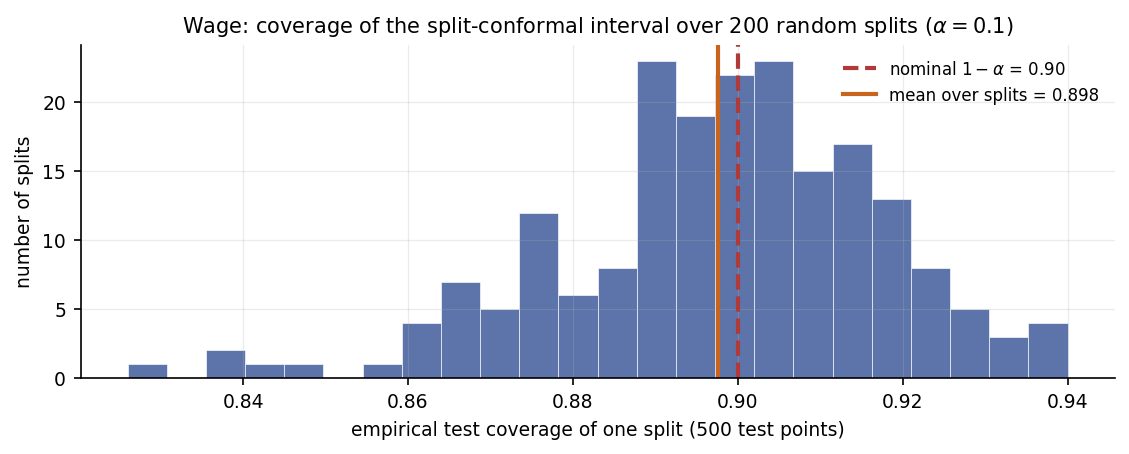
\includegraphics[width=0.88\textwidth,height=0.55\textheight,keepaspectratio]{a3_coverage_hist.png}
  \end{center}
  \begin{takeaway}
    200 random splits of Wage: per-split test coverage fluctuates between $0.826$ and
    $0.940$ (sd $0.020$), but the \emph{mean} is $0.898 \approx 0.9$ --- the marginal
    guarantee in action. Any \emph{single} split can land at $0.87$; nothing is wrong
    when it does.
  \end{takeaway}
  \begin{labnote}[Notebook \S2: coverage over repeated splits]
    \S2 re-runs the split 200 times and reproduces this histogram --- mean $0.8976$,
    sd $0.0198$. The appendix derives why the spread is exactly of this size.
  \end{labnote}
\end{frame}

\begin{frame}{The honest slide: marginal is not conditional}
  \begin{center}
    
\includegraphics[width=0.74\textwidth,height=0.5\textheight,keepaspectratio]{a3_subgroup.png}
  \end{center}
  \begin{takeaway}
    Same interval, same split: coverage is $98.6\%$ for under-30s but only $82.9\%$
    for the 60-plus group --- the marginal $92.6\%$ is an \emph{average} that hides
    both. A constant-width band overcovers where wages are predictable and
    undercovers where they spread out.
  \end{takeaway}
  \begin{mistake}
    Promising a customer segment ``90\% coverage'' because the overall model is
    conformal. Per-subgroup coverage is \textbf{not} guaranteed --- if a group matters,
    calibrate on that group (Mondrian conformal, appendix) or use adaptive scores
    (next section).
  \end{mistake}
\end{frame}

% ------------------------------------------------------------
\begin{frame}{Exercise A3.3 --- How small can the calibration set be? [Math]}
\begin{exercise}
  The conformal index is $k = \lceil (n+1)(1-\alpha) \rceil$, and $\hat q = s_{(k)}$
  only exists if $k \le n$.
  \begin{enumerate}
    \item Show that $k \le n$ is equivalent to
          $n \ge \tfrac{1-\alpha}{\alpha} = \tfrac{1}{\alpha} - 1$.
    \item Evaluate the minimal $n$ for $\alpha = 0.1$, $0.05$, and $0.01$.
    \item A team calibrates with $n = 10$ points at $\alpha = 0.05$. What interval
          does the recipe return, and why is that the honest answer?
    \item Which coverage levels are \emph{exactly} achievable with $n = 9$?
  \end{enumerate}
\end{exercise}
\end{frame}

\begin{frame}{Solution --- Exercise A3.3}
\begin{solutionbox}
  \textbf{Method.} Unpack the ceiling: $k \le n \iff (n+1)(1-\alpha) \le n$.
  \begin{itemize}
    \item \textbf{Part 1.} $(n+1)(1-\alpha) \le n
          \iff n + 1 - \alpha n - \alpha \le n
          \iff 1 - \alpha \le \alpha n
          \iff n \ge \tfrac{1-\alpha}{\alpha} = \tfrac{1}{\alpha} - 1$. $\checkmark$
    \item \textbf{Part 2.} $\alpha = 0.1$: $n \ge 9$. \quad $\alpha = 0.05$:
          $n \ge 19$. \quad $\alpha = 0.01$: $n \ge 99$.
    \item \textbf{Part 3.} $k = \lceil 11 \times 0.95 \rceil = \lceil 10.45 \rceil
          = 11 > 10$: there is no 11th score, so
          $\hat q = \infty$ and $C(x) = (-\infty, \infty)$. Honest, because with 10
          exchangeable scores the new point exceeds \emph{all} of them with probability
          $1/11 \approx 9.1\% > 5\%$ --- no finite cut-off can promise 95\%.
    \item \textbf{Part 4.} Achievable exact levels are $\tfrac{k}{n+1} = \tfrac{k}{10}$:
          $10\%, 20\%, \dots, 90\%, 100\%$ --- coverage is \emph{quantized} in steps of
          $\tfrac{1}{n+1}$.
  \end{itemize}
\end{solutionbox}
\begin{mistake}
  Requesting $\alpha = 0.01$ from $n = 50$ calibration points and ``fixing'' the
  infinite interval by switching to the plain empirical maximum. The interval is then
  no longer guaranteed --- collect more calibration data instead.
\end{mistake}
\end{frame}

% ============================================================
\section{Adaptive Intervals}
% ============================================================

\begin{frame}{One width for everyone is a blunt instrument}
  The absolute-residual band on Wage is $\pm 56.1$ \emph{everywhere}: for 20-year-olds
  (tightly clustered wages) and for 60-year-olds (wide spread) alike.
  \begin{readme}[Two ways to make the width follow the data]
    \begin{itemize}
      \item \textbf{Locally weighted scores}: fit a second model
            $\hat\sigma(x)$ for the typical error size, and score
            \[
              s_i = \frac{|y_i - \hat f(x_i)|}{\hat\sigma(x_i)}
              \qquad\Longrightarrow\qquad
              C(x) = \hat f(x) \pm \hat q\, \hat\sigma(x).
            \]
      \item \textbf{Conformalized quantile regression (CQR)}: model the
            \emph{quantiles} of $Y \mid X$ directly, then calibrate them.
    \end{itemize}
    Both keep the marginal guarantee --- any fixed score function works, because the
    scores of exchangeable points remain exchangeable.
  \end{readme}
  \begin{numexample}[Locally weighted conformal on Wage]
    $\hat\sigma(x)$: quadratic fit of $|$residual$|$ on age. Result:
    $\hat q = 1.90$ (in $\sigma$-units), test coverage $89.6\%$, and widths now range
    from $42$ (age 18) to $121$ (age 50) instead of a flat $112$.
  \end{numexample}
\end{frame}

\begin{frame}[fragile]{The engine: quantile regression with the pinball loss}
  \begin{block}{Pinball (quantile) loss at level $\tau$}
    \[
      \rho_\tau(u) =
      \begin{cases}
        \tau\, u & u \ge 0 \\
        (\tau - 1)\, u & u < 0
      \end{cases}
      \qquad u = y - q .
    \]
    Minimising $E\,\rho_\tau\big(Y - q(X)\big)$ over functions $q$ yields the
    conditional $\tau$-quantile of $Y \mid X$.
  \end{block}
  \begin{readme}[Why it works --- in one sentence]
    Undershooting costs $\tau$ per unit, overshooting costs $1 - \tau$: the optimal
    $q(x)$ sits where a fraction $\tau$ of the mass lies below --- exactly the
    quantile. At $\tau = 0.5$ it is the absolute loss, and we recover the median.
  \end{readme}
  \begin{lstlisting}
from sklearn.ensemble import GradientBoostingRegressor   # Ch. 8 engine
lo = GradientBoostingRegressor(loss="quantile", alpha=0.05,   # 5% curve
        n_estimators=200, max_depth=2, learning_rate=0.05)
hi = GradientBoostingRegressor(loss="quantile", alpha=0.95,   # 95% curve
        n_estimators=200, max_depth=2, learning_rate=0.05)
  \end{lstlisting}
\end{frame}

\begin{frame}{Conformalized quantile regression (CQR)}
  \begin{block}{Algorithm (Romano, Patterson \& Cand\`es, 2019)}
    \begin{enumerate}
      \item On $\mathcal{D}_{\text{tr}}$, fit quantile curves
            $\hat q_{\text{lo}}$ (level $\alpha/2$) and $\hat q_{\text{hi}}$
            (level $1 - \alpha/2$).
      \item On $\mathcal{D}_{\text{cal}}$, score
            $\;\boxed{\;s_i = \max\big(\hat q_{\text{lo}}(x_i) - y_i,\;
            y_i - \hat q_{\text{hi}}(x_i)\big)\;}$
      \item $\hat q = s_{(k)}$ with the usual $k = \lceil (n+1)(1-\alpha) \rceil$; report
            $C(x) = \big[\hat q_{\text{lo}}(x) - \hat q,\;
            \hat q_{\text{hi}}(x) + \hat q\big]$.
    \end{enumerate}
  \end{block}
  \begin{readme}[Decoding the score]
    $s_i$ is the \emph{signed distance to the nearer violated edge}: positive if
    $y_i$ falls outside $[\hat q_{\text{lo}}, \hat q_{\text{hi}}]$ (by how much),
    \emph{negative} if inside (how deep). If the fitted band already overcovers,
    $\hat q < 0$ \emph{shrinks} it; if it undercovers, $\hat q > 0$ pads it. Same
    quantile index, same guarantee --- the width now lives in the quantile curves.
  \end{readme}
  \begin{takeaway}
    CQR = ``let Chapter 8 draw the band, let conformal calibrate it''. On Wage the
    correction is tiny: $\hat q = 0.66$ --- the boosted 5\%/95\% curves were almost
    calibrated already.
  \end{takeaway}
\end{frame}

\begin{frame}{Wage: constant width vs adaptive width}
  \begin{center}
    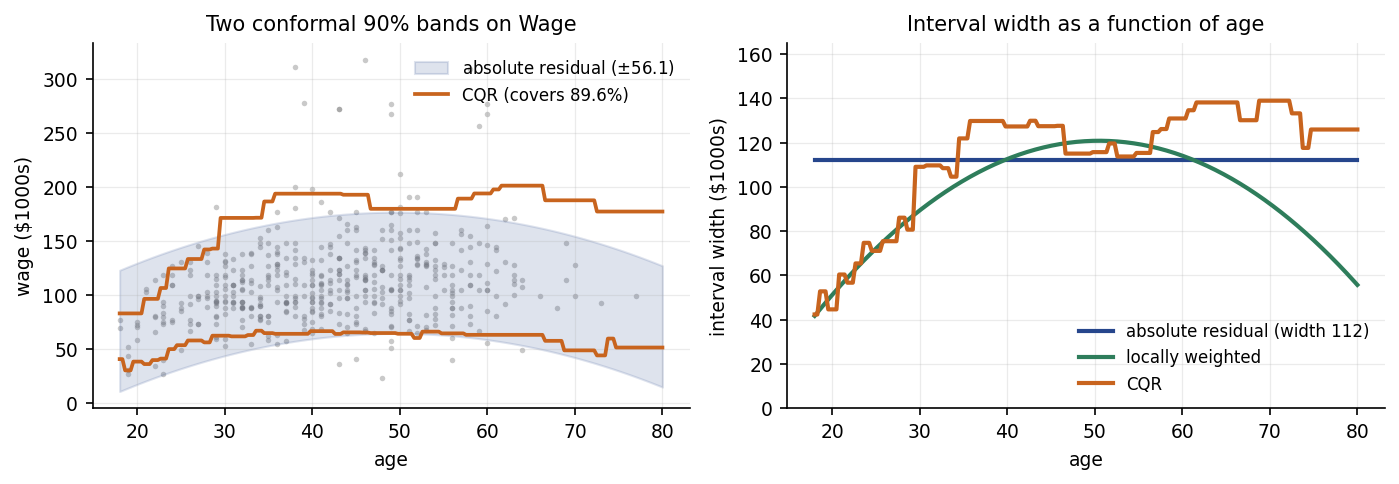
\includegraphics[width=0.94\textwidth,height=0.55\textheight,keepaspectratio]{a3_cqr.png}
  \end{center}
  \begin{takeaway}
    Both bands cover $\approx 90\%$ marginally (CQR: $89.6\%$), but CQR spends its
    width where the data spread: average width $70.5$ for under-30s vs $134.9$ for
    60-plus (constant band: $112.3$ for both). Note the locally weighted curve
    \emph{falls} after age 60 --- its quadratic $\hat\sigma$ extrapolates poorly: the
    allocation is only as good as the scale model, even though marginal coverage
    ($89.6\%$) is untouched.
  \end{takeaway}
  \begin{labnote}[Notebook \S3: adaptive intervals]
    \S3 fits both adaptive variants and reproduces this figure's numbers:
    $\hat q_{\text{lw}} = 1.897$, $\hat q_{\text{cqr}} = 0.66$, and the three width
    profiles.
  \end{labnote}
\end{frame}

% ------------------------------------------------------------
\begin{frame}{Extended Exercise A3.1 --- CQR on Wage, end to end [Python]}
\begin{longexercise}
  Reproduce the adaptive band. Using the deck's split of \texttt{Wage}
  (seed 2024; $2\,000$ / $500$ / $500$):
  \begin{enumerate}
    \item Fit \texttt{GradientBoostingRegressor(loss="quantile")} at levels $0.05$
          and $0.95$ on the training set (200 trees, depth 2, learning rate 0.05,
          \texttt{random\_state=0}).
    \item Compute the CQR scores on the calibration set and $\hat q$ at
          $\alpha = 0.1$; report test coverage.
    \item Compare average interval width for ages $<30$, $30$--$59$ and $\ge 60$
          against the constant-width band ($112.3$).
    \item Compare the two bands' \emph{subgroup coverage} for under-30s and 60-plus.
          Which failure of the constant band does CQR repair, and what does it
          \emph{not} guarantee?
  \end{enumerate}
\end{longexercise}
\begin{labnote}[Run this live]
  The worked solution sits in \texttt{advanced\_03\_conformal\_lab.ipynb} under
  \emph{Lecture exercises --- worked Python solutions}: the cell headed
  \emph{Extended Exercise A3.1 --- CQR on Wage, end to end [Python]}.
\end{labnote}
\end{frame}

\begin{frame}[fragile]{Solution --- Extended Exercise A3.1 (1/2)}
\begin{solutionbox}[Solution --- code: fit / score / calibrate]
\begin{lstlisting}[basicstyle=\ttfamily\scriptsize]
import numpy as np, pandas as pd                     # data handling
from sklearn.ensemble import GradientBoostingRegressor

wage = pd.read_csv("Wage.csv")                       # lab: via load()
x, y = wage["age"].to_numpy(float), wage["wage"].to_numpy()
rng = np.random.default_rng(2024)                    # the deck's split
i = rng.permutation(len(y)); tr, ca, te = i[:2000], i[2000:2500], i[2500:]
X = x.reshape(-1, 1)
gb = dict(n_estimators=200, max_depth=2, learning_rate=0.05, random_state=0)
lo = GradientBoostingRegressor(loss="quantile", alpha=0.05, **gb).fit(X[tr], y[tr])
hi = GradientBoostingRegressor(loss="quantile", alpha=0.95, **gb).fit(X[tr], y[tr])
s = np.maximum(lo.predict(X[ca]) - y[ca], y[ca] - hi.predict(X[ca]))  # CQR score
k = int(np.ceil((len(ca) + 1) * 0.9))                # k = 451
qhat = np.sort(s)[k - 1]                             # 0.66: tiny correction
L, U = lo.predict(X[te]) - qhat, hi.predict(X[te]) + qhat
print(round(qhat, 2), ((y[te] >= L) & (y[te] <= U)).mean())  # 0.66 0.896
\end{lstlisting}
\end{solutionbox}
\end{frame}

\begin{frame}{Solution --- Extended Exercise A3.1 (2/2)}
\begin{solutionbox}[Solution --- numbers and interpretation]
  \textbf{Parts 2--3.} $\hat q = 0.66$; test coverage $= 0.896$. Average widths:
  \begin{center}
  \footnotesize
  \begin{tabular}{@{}lccc@{}}
    \toprule
    & age $<30$ & age 30--59 & age $\ge 60$ \\
    \midrule
    Constant band (abs.\ residual) & $112.3$ & $112.3$ & $112.3$ \\
    CQR band & $70.5$ & $120.4$ & $134.9$ \\
    \bottomrule
  \end{tabular}
  \end{center}
  \textbf{Part 4.} Subgroup coverage on this split: constant band $0.986$ (under-30)
  vs $0.829$ (60-plus); CQR $0.797$ vs $0.886$. CQR repairs the \emph{width
  misallocation} --- it stops wasting $40$ units of width on the young and reinvests
  them in the old, whose coverage rises from $0.829$ to $0.886$.
  \textbf{What it does not guarantee:} exact per-group coverage --- the young bin
  ($n = 74$) lands at $0.797$ here, within sampling noise of $0.9$ but not pinned to
  it. Only the \emph{marginal} $90\%$ is guaranteed; per-group guarantees need
  per-group calibration.
\end{solutionbox}
\begin{mistake}
  Fitting $\hat q_{\text{lo}}, \hat q_{\text{hi}}$ on training \emph{plus} calibration
  data ``to use all the data''. The scores are then not exchangeable with the test
  score, and the guarantee is void --- the split is load-bearing.
\end{mistake}
\end{frame}

% ============================================================
\section{Conformal Classification}
% ============================================================

\begin{frame}{From intervals to prediction sets}
  For a classifier there is no interval --- the honest object is a \textbf{set of
  classes} $C(x) \subseteq \{1, \dots, K\}$.
  \begin{block}{Split conformal for classification}
    \begin{enumerate}
      \item Fit a probabilistic classifier $\hat p$ on $\mathcal{D}_{\text{tr}}$
            (e.g.\ softmax / logistic regression, Ch.\ 4).
      \item Calibration scores: $\;\boxed{\;s_i = 1 - \hat p_{y_i}(x_i)\;}$ --- one
            minus the probability assigned to the \emph{true} class.
      \item $\hat q = s_{(k)}$, $k = \lceil (n+1)(1-\alpha) \rceil$ as always; report
            \[
              C(x) = \big\{\,k :\; \hat p_k(x) \ge 1 - \hat q \,\big\}.
            \]
      \end{enumerate}
  \end{block}
  \begin{readme}[Decoding the set rule]
    A class enters the set when its softmax probability clears the threshold
    $1 - \hat q$. Confident points get \textbf{singletons}; ambiguous points near a
    decision boundary get $\{1, 2\}$ or bigger. The guarantee: the \emph{true} class
    is in $C(X)$ with probability $\ge 1 - \alpha$ --- same rank argument, unchanged.
  \end{readme}
\end{frame}

\begin{frame}{A 3-class simulation: sets earn their keep at the boundaries}
  \begin{center}
    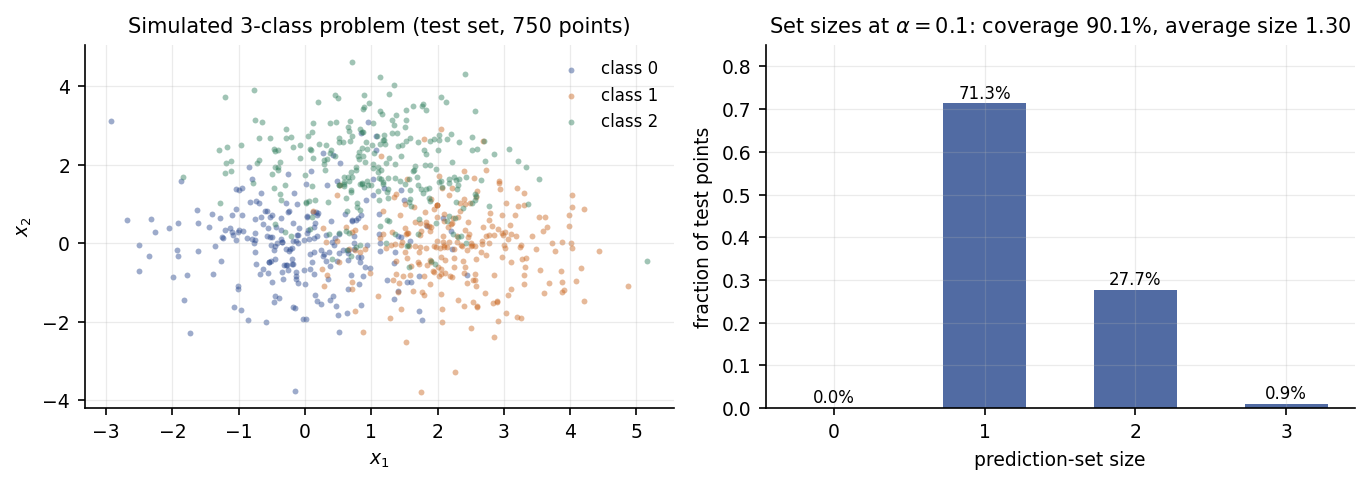
\includegraphics[width=0.92\textwidth,height=0.55\textheight,keepaspectratio]{a3_three_class.png}
  \end{center}
  \begin{takeaway}
    Three Gaussian classes (centres $(0,0)$, $(2.2,0)$, $(1.1,1.9)$; logistic
    accuracy $80.9\%$). At $\alpha = 0.1$: $\hat q = 0.7685$ (score 676 of 750),
    coverage $90.1\%$, average set size $1.30$ --- $71.3\%$ singletons, $27.7\%$
    pairs, $0.9\%$ full sets. The set \emph{size} is a per-point difficulty meter the
    accuracy number hides.
  \end{takeaway}
  \begin{labnote}[Notebook \S4: conformal classification]
    \S4 simulates these three classes (seed 2024), builds the sets and reproduces
    coverage $0.9013$ and the size distribution above.
  \end{labnote}
\end{frame}

\begin{frame}{The price of certainty: coverage vs set size}
  \begin{center}
    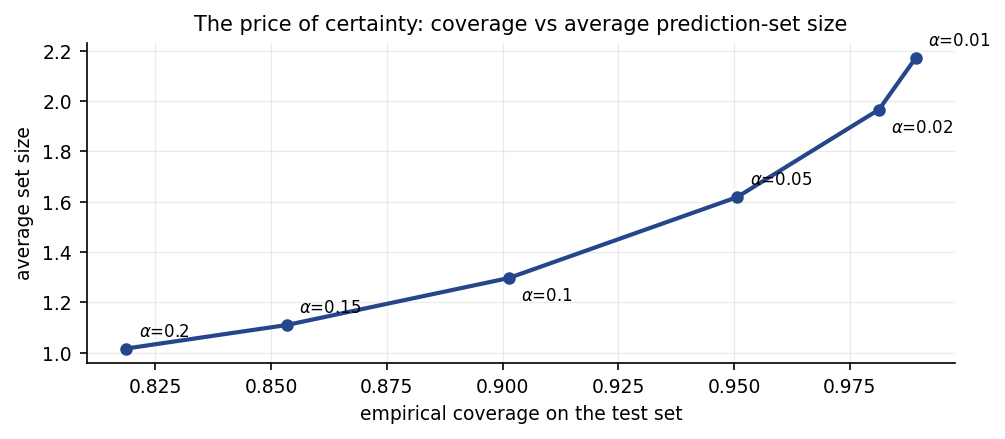
\includegraphics[width=0.7\textwidth,height=0.5\textheight,keepaspectratio]{a3_tradeoff.png}
  \end{center}
  \begin{takeaway}
    Demanding $99\%$ coverage inflates the average set from $1.30$ to $2.17$ classes
    --- two-thirds of the label space. Certainty is bought with set size; pick
    $\alpha$ by what a large set \emph{costs downstream} (a manual review, a second
    lab test).
  \end{takeaway}
  \begin{readme}[One slide on APS (adaptive prediction sets)]
    The $1 - \hat p$ score judges each class alone, so it can return \emph{empty} sets
    when $\alpha$ is loose (here: $0.9\%$ empty at $\alpha = 0.2$) and adapts poorly
    across easy/hard regions. \textbf{APS} scores the \emph{cumulative} probability
    mass needed to reach the true class (add classes in decreasing $\hat p_k$); sets
    are never empty and track difficulty better, at the price of being larger on
    average. Same calibration machinery.
  \end{readme}
\end{frame}

% ------------------------------------------------------------
\begin{frame}{Exercise A3.4 --- Reading prediction sets [Concept]}
\begin{exercise}
  A conformal classifier ($K = 3$, $\alpha = 0.1$) was calibrated with
  $\hat q = 0.7685$, so classes enter the set when $\hat p_k(x) \ge 0.2315$.
  Three test customers get softmax probabilities:
  \[
    \text{A: } (0.95,\ 0.03,\ 0.02) \qquad
    \text{B: } (0.50,\ 0.45,\ 0.05) \qquad
    \text{C: } (0.40,\ 0.35,\ 0.25)
  \]
  \begin{enumerate}
    \item Write down the prediction set of each customer.
    \item The plain classifier predicts class 0 for all three. What extra information
          do the sets carry?
    \item Can the guarantee be read as ``$90\%$ of \emph{singleton} sets are
          correct''? Why not?
    \item Under which circumstances can the rule return an \emph{empty} set, and what
          should a production system do with one?
  \end{enumerate}
\end{exercise}
\end{frame}

\begin{frame}{Solution --- Exercise A3.4}
\begin{solutionbox}
  \textbf{Method.} Threshold each probability at $1 - \hat q = 0.2315$.
  \begin{itemize}
    \item \textbf{Part 1.} A: $\{0\}$ ($0.95$ clears, others do not). B: $\{0, 1\}$
          ($0.50$ and $0.45$ clear). C: $\{0, 1, 2\}$ (all three $\ge 0.2315$).
    \item \textbf{Part 2.} Identical point predictions, very different epistemic
          states: A is settled, B is a genuine two-way toss-up, C is anyone's guess.
          The set size is the honest ``how sure are we'' channel a point prediction
          lacks.
    \item \textbf{Part 3.} No. The guarantee is \emph{marginal over all points}:
          $\ge 90\%$ of \emph{all} sets contain the truth. Singletons are the
          \emph{easy} points, so their hit rate is typically above $90\%$, while the
          large sets carry more of the mistakes --- but neither is individually
          guaranteed.
    \item \textbf{Part 4.} Empty sets occur when even the largest probability misses
          the threshold: possible once $\hat q < 1 - \max_k \hat p_k(x)$, i.e.\ with
          loose $\alpha$ and diffident models (our simulation: $0.9\%$ empty at
          $\alpha = 0.2$, none at $\alpha = 0.1$). Production systems treat empty
          (like oversized) sets as \textbf{abstentions}: route to a human.
  \end{itemize}
\end{solutionbox}
\begin{mistake}
  Treating the set as a ranking. $C(x)$ is an \emph{unordered} guarantee region ---
  ``class 0 first'' is the old point prediction sneaking back in.
\end{mistake}
\end{frame}

% ============================================================
\section{Conformal vs Classical}
% ============================================================

\begin{frame}{Same data, two intervals: when the model is right, they agree}
  \begin{numexample}[Homoskedastic simulation --- the friendly case]
    $y = 1 + 2x + \varepsilon$, $\varepsilon \sim \mathcal{N}(0, 2^2)$,
    $x \sim U(0, 10)$; $2\,000$ training, $1\,000$ calibration, $1\,000$ test points
    (seed 2024). Theory: 90\% half-width $= 1.645 \times 2 = 3.29$.
    \begin{center}
    \footnotesize
    \begin{tabular}{@{}lcc@{}}
      \toprule
      & half-width & test coverage \\
      \midrule
      OLS prediction interval (Ch.\ 3) & $3.31$ & $0.915$ \\
      Split conformal (abs.\ residual) & $3.24$ & $0.909$ \\
      \bottomrule
    \end{tabular}
    \end{center}
  \end{numexample}
  \begin{takeaway}
    When the Gaussian linear model is \emph{true}, conformal costs essentially
    nothing: both intervals reproduce the theoretical $\pm 3.29$. Conformal is not a
    better interval --- it is the same interval with a \emph{weaker warranty
    requirement}.
  \end{takeaway}
  \begin{industry}[Model risk management: two numbers as one sanity check]
    Validation teams in banking run both: if the parametric and the conformal interval
    disagree materially, the \emph{model assumptions} are the prime suspect --- a
    cheap, assumption-free diagnostic.
  \end{industry}
\end{frame}

\begin{frame}{Heteroskedastic truth: where the 90\% quietly stops being 90\%}
  \begin{center}
    
\includegraphics[width=0.94\textwidth,height=0.55\textheight,keepaspectratio]{a3_hetero.png}
  \end{center}
  \begin{takeaway}
    $y = 1 + 2x + x\,\varepsilon$: noise grows with $x$. All three methods hold
    $\approx 90\%$ \emph{marginally} (OLS $0.906$, conformal $0.908$, CQR $0.906$)
    --- but conditionally the constant-width pair collapses to $\mathbf{73.5\%}$
    ($74.1\%$) for $x > 8$ while overcovering at $100\%$ for $x < 2$. Only CQR stays
    near $0.90$ in \emph{every} bin ($0.916$ to $0.899$). And only conformal
    \emph{guarantees} its marginal number: over 100 repeated simulations, OLS averages
    $0.894$ (luck, no warranty), conformal $0.900$ (by theorem).
  \end{takeaway}
\end{frame}

\begin{frame}{The failure that actually happens: plug-in intervals from a flexible model}
  \begin{numexample}[Same heteroskedastic data --- boosted regression]
    Fit a 500-tree gradient boosting model, then do what practitioners actually do:
    $\hat f(x) \pm 1.645 \times \hat\sigma_{\text{in}}$ with $\hat\sigma_{\text{in}}$
    the sd of the \emph{training} residuals.
    \begin{center}
    \footnotesize
    \begin{tabular}{@{}lccc@{}}
      \toprule
      & $\hat\sigma$ used & claimed & actual test coverage \\
      \midrule
      Plug-in (training residuals) & $3.92$ & $90\%$ & $\mathbf{77.6\%}$ \\
      Split conformal (same model) & $\hat q = 10.81$ & $\ge 90\%$ & $90.7\%$ \\
      \bottomrule
    \end{tabular}
    \end{center}
    The truth: held-out residual sd is $6.12$ --- the model memorised a third of the
    noise, and the plug-in interval inherited the optimism.
  \end{numexample}
  \begin{mistake}
    Calibrating interval width on data the model has seen. Training residuals of a
    flexible model are systematically too small; every per-cent of memorised noise is
    a per-cent of silent undercoverage. The conformal split exists precisely to make
    this mistake impossible.
  \end{mistake}
\end{frame}

\begin{frame}{Chapter 3's interval vs split conformal --- the comparison slide}
  \footnotesize
  \begin{center}
  \begin{tabular}{@{}p{3.4cm}p{4.5cm}p{4.7cm}@{}}
    \toprule
    & \textbf{OLS prediction interval} & \textbf{Split conformal} \\
    \midrule
    Assumes & linear mean, Gaussian, homoskedastic errors & exchangeability + a clean
      split \\
    Guarantee & exact at every $x$, \emph{if} the model is true & marginal
      $\ge 1 - \alpha$, finite-sample, \emph{whatever} the model \\
    Works with & the linear model it was derived for & any $\hat f$: boosting, nets,
      black boxes \\
    Width & $\approx$ constant ($\hat\sigma$-driven; slightly wider at high leverage)
      & constant (abs.\ residual) or adaptive (CQR) \\
    Cost & none & holds out $n$ calibration points \\
    Under misspecification & silently wrong coverage & coverage intact; only width
      reacts \\
    \bottomrule
  \end{tabular}
  \end{center}
  \begin{takeaway}
    Use the OLS interval when you \emph{believe} the Gaussian linear model and want
    conditional statements. Use conformal when the model is flexible, the errors are
    ugly, or the coverage number will be \emph{audited}.
  \end{takeaway}
\end{frame}

% ------------------------------------------------------------
\begin{frame}{Extended Exercise A3.2 --- Stress-testing the two intervals [Integrative]}
\begin{longexercise}
  Simulate $y = 1 + 2x + x\,\varepsilon$, $\varepsilon \sim \mathcal{N}(0,1)$,
  $x \sim U(0, 10)$, $n = 4\,000$ (split $2\,000$ / $1\,000$ / $1\,000$, seed 2024).
  \begin{enumerate}
    \item Fit OLS on the training set; build the 90\% prediction interval
          $\hat y \pm 1.645\,\hat\sigma$ and measure test coverage overall, for
          $x < 2$, and for $x > 8$.
    \item Build the split-conformal interval (absolute residuals, $\alpha = 0.1$) and
          measure the same three coverages. What does conformal fix here --- and what
          does it not fix?
    \item Fit a 500-tree \texttt{GradientBoostingRegressor}; report coverage of
          $\hat f \pm 1.645 \times \text{sd(training residuals)}$, then conformalise
          the same model. Explain the mechanism behind the gap.
    \item Conclude: which of the three failure modes (skewed errors, heteroskedastic
          errors, optimistic $\hat\sigma$) does split conformal repair marginally,
          and which needs CQR?
  \end{enumerate}
\end{longexercise}
\begin{labnote}[Run this live]
  Worked solution in \texttt{advanced\_03\_conformal\_lab.ipynb} under \emph{Lecture
  exercises --- worked Python solutions}, cell \emph{Extended Exercise A3.2}.
\end{labnote}
\end{frame}

\begin{frame}[fragile]{Solution --- Extended Exercise A3.2 (1/2)}
\begin{solutionbox}[Solution --- code: the three intervals]
\begin{lstlisting}[basicstyle=\ttfamily\scriptsize]
import numpy as np, statsmodels.api as sm
from sklearn.ensemble import GradientBoostingRegressor
rng = np.random.default_rng(2024)
N = 4000; x = rng.uniform(0, 10, N); y = 1 + 2*x + x*rng.normal(0, 1, N)
tr, ca, te = np.arange(2000), np.arange(2000, 3000), np.arange(3000, 4000)
ols = sm.OLS(y[tr], sm.add_constant(x[tr])).fit()      # 1. classical PI
half = 1.645 * np.sqrt(ols.scale)                      # pooled sigma: 5.87
pred = ols.params[0] + ols.params[1] * x[te]
cov = lambda hit: [hit.mean(), hit[x[te] < 2].mean(), hit[x[te] > 8].mean()]
print(cov(np.abs(y[te] - pred) <= half))               # [0.906, 1.000, 0.735]
k = int(np.ceil(1001 * 0.9))                           # 2. conformal: k = 901
q = np.sort(np.abs(y[ca] - (ols.params[0] + ols.params[1]*x[ca])))[k-1]
print(q, cov(np.abs(y[te] - pred) <= q))               # 9.8 [0.908, 1.0, 0.741]
f = GradientBoostingRegressor(n_estimators=500, random_state=0)  # 3. plug-in
f.fit(x[tr, None], y[tr]); sig = np.std(y[tr] - f.predict(x[tr, None]))  # 3.92
print(cov(np.abs(y[te] - f.predict(x[te, None])) <= 1.645 * sig))  # [0.776, ...]
qg = np.sort(np.abs(y[ca] - f.predict(x[ca, None])))[k-1]          # 10.81
print(cov(np.abs(y[te] - f.predict(x[te, None])) <= qg))           # [0.907, ...]
\end{lstlisting}
\end{solutionbox}
\end{frame}

\begin{frame}{Solution --- Extended Exercise A3.2 (2/2)}
\begin{solutionbox}[Solution --- interpretation]
  \textbf{Part 1.} OLS: marginal $0.906$, but $100\%$ for $x < 2$ and $73.5\%$ for
  $x > 8$ --- the pooled $\hat\sigma = 5.87$ is one compromise width for noise that
  ranges from $\approx 0$ to $10$.
  \textbf{Part 2.} Conformal ($\hat q = 9.79$): marginal $0.908$, subgroups $1.00$ /
  $0.741$ --- conformal \emph{guarantees the marginal number} (over repeated data:
  $0.900$ vs OLS's drifting $0.894$) but a constant-width score cannot repair the
  \emph{conditional} imbalance. That is CQR's job (it reaches $0.899$ at $x > 8$).
  \textbf{Part 3.} Plug-in GBR: claimed $90\%$, actual $\mathbf{77.6\%}$ ---
  training-residual sd ($3.92$) understates held-out error sd ($6.12$) because the
  500-tree model partly memorised the training noise. Conformalising the \emph{same}
  model restores $90.7\%$ by pricing the width on unseen data ($\hat q = 10.81$).
  \textbf{Part 4.} Marginal repairs come free (skew, heteroskedasticity, optimism all
  handled --- the guarantee never moved); \emph{conditional} honesty across $x$ is the
  one thing that needs an adaptive score (CQR / locally weighted).
\end{solutionbox}
\begin{mistake}
  Concluding from part 2 that conformal ``failed''. It delivered exactly what it
  promises --- marginal coverage; expecting per-region coverage from a constant-width
  score is a specification error, not a method error.
\end{mistake}
\end{frame}

% ============================================================
\section{Pitfalls and Practice}
% ============================================================

\begin{frame}{Pitfall 1: exchangeability violations in the wild}
  \begin{itemize}
    \item \textbf{Time series}: calibration residuals from a five-year window,
          deployment two years later --- trends, seasonality and regime shifts make the test point
          \emph{special}, which is exactly what exchangeability forbids.
    \item \textbf{Covariate shift}: a marketing model calibrated on organic traffic,
          deployed during a paid campaign --- the $X$-mix changed overnight.
    \item \textbf{Selection feedback}: the model approves loans, and only approved
          loans generate future calibration labels.
  \end{itemize}
  \begin{readme}[What to do instead]
    Time series: calibrate on the \emph{most recent} block, recalibrate on a schedule,
    or use online/adaptive conformal that tunes $\alpha$ from realised coverage.
    Known covariate shift: \emph{weighted} conformal with likelihood-ratio weights
    $w(x) = p_{\text{new}}(x)/p_{\text{cal}}(x)$. Always: monitor realised coverage
    --- the guarantee you can check is the one you keep.
  \end{readme}
  \begin{industry}[Energy trading: recalibrate with the seasons]
    A wind-power desk recalibrates its forecast intervals \emph{daily} on the trailing
    30 days. A fixed calibration set from spring undercovers in autumn storms ---
    same model, dead guarantee.
  \end{industry}
\end{frame}

\begin{frame}{Pitfall 2: leakage between fitting and calibration}
  The guarantee has exactly one hard requirement inside your pipeline:
  \emph{nothing about $\hat f$ may depend on the calibration set}.
  \begin{readme}[The four common leak channels]
    \begin{enumerate}
      \item \textbf{Preprocessing}: scaler / imputer / encoder fit on \emph{all} data
            before the split.
      \item \textbf{Tuning}: hyperparameters or early stopping selected on calibration
            performance.
      \item \textbf{Feature selection}: screening variables on the full sample
            (the Ch.\ 5 classic).
      \item \textbf{Duplicates}: the same customer's rows on both sides of the split.
    \end{enumerate}
    Each one shrinks calibration scores below test scores $\Rightarrow$ $\hat q$ too
    small $\Rightarrow$ silent undercoverage --- the plug-in GBR's $77.6\%$ was this
    mechanism in its purest form.
  \end{readme}
  \begin{mistake}
    ``Refitting on train + calibration after computing $\hat q$, since the interval is
    already fixed.'' The deployed $\hat f$ is then not the one that generated the
    scores --- the pair $(\hat f, \hat q)$ is calibrated \emph{together} or not at all.
  \end{mistake}
\end{frame}

\begin{frame}{From ten lines to production}
  \begin{readme}[Practical sizing rules]
    \begin{itemize}
      \item \textbf{Feasibility}: $\alpha$ needs $n \ge \tfrac{1}{\alpha} - 1$
            (19 points for 95\%, 99 for 99\%) --- below that the honest interval is
            infinite (Exercise A3.3).
      \item \textbf{Stability}: with $n = 500$ the coverage of one split has sd
            $\approx 1.3\%$ (appendix); $n$ between 500 and $1\,000$ is the usual
            sweet spot --- beyond that, spend the data on training.
      \item \textbf{Report the nature of the guarantee}: marginal, at the stated
            $\alpha$, under exchangeability --- three words that pre-empt three
            misreadings.
    \end{itemize}
  \end{readme}
  \begin{industry}[Tooling: MAPIE and friends]
    In production, teams reach for \textbf{MAPIE} (\emph{Model Agnostic Prediction
    Interval Estimator}, scikit-learn compatible): split/cross conformal,
    CQR and classification sets behind one API, plus jackknife+ variants that recycle
    training folds. It is not installed here --- deliberately: everything in this
    module was ten lines from scratch, and those ten lines are the audit trail you
    will be asked for.
  \end{industry}
\end{frame}

% ============================================================
\section{Python Lab}
% ============================================================

\begin{frame}{Python lab --- run it live in the notebook}
  \begin{labnote}[Companion notebook: \texttt{advanced\_03\_conformal\_lab.ipynb}]
    The code in this section is meant to be \textbf{demonstrated live}. Open the
    companion Jupyter notebook and run it cell by cell:
    \begin{itemize}
      \item \S1, \emph{Split conformal on Wage} --- the ten-line recipe:
            $\hat q = 56.14$, coverage $0.926$;
      \item \S2, \emph{Coverage over repeated splits} --- 200 splits, mean $0.898$;
      \item \S3, \emph{Adaptive intervals} --- locally weighted scores and CQR,
            width profiles by age;
      \item \S4, \emph{Conformal classification} --- 3-class simulation, prediction
            sets, size distribution;
      \item \S5, \emph{OLS prediction interval vs conformal} --- the heteroskedastic
            stress test.
    \end{itemize}
    Data loads via the \texttt{ISLP} package or the bundled CSV files; \S6,
    \emph{Exercises} ends the notebook with hands-on tasks.
  \end{labnote}
\end{frame}

\begin{frame}[fragile]{Split conformal in ten lines}
  \begin{lstlisting}
import numpy as np, pandas as pd
from sklearn.linear_model import LinearRegression

wage = pd.read_csv("Wage.csv")                       # lab: via load()
x, y = wage["age"].to_numpy(float), wage["wage"].to_numpy()
rng = np.random.default_rng(2024)                    # reproducible split
i = rng.permutation(len(y)); tr, ca, te = i[:2000], i[2000:2500], i[2500:]
P = lambda a: np.column_stack([a, a**2])             # quadratic in age
f = LinearRegression().fit(P(x[tr]), y[tr])          # 1. fit on TRAIN only
s = np.abs(y[ca] - f.predict(P(x[ca])))              # 2. calibration scores
k = int(np.ceil((len(ca) + 1) * (1 - 0.1)))          # 3. k = ceil((n+1)(1-a))
qhat = np.sort(s)[k - 1]                             #    k-th smallest score
cov = (np.abs(y[te] - f.predict(P(x[te]))) <= qhat).mean()  # 4. check
print(k, qhat.round(2), cov)                         # 451 56.14 0.926
  \end{lstlisting}
\end{frame}

% ------------------------------------------------------------
\begin{frame}{Exercise A3.5 --- Conformal classification from scratch [Python]}
\begin{exercise}
  Build prediction sets for the deck's 3-class simulation (three Gaussian classes,
  $1\,000$ points each, centres $(0,0)$, $(2.2, 0)$, $(1.1, 1.9)$, unit variance,
  seed 2024; split $1\,500$ / $750$ / $750$).
  \begin{enumerate}
    \item Fit \texttt{LogisticRegression} on the training set.
    \item Compute the calibration scores $s_i = 1 - \hat p_{y_i}(x_i)$ and $\hat q$
          at $\alpha = 0.1$ (which $k$?).
    \item Build the test-set prediction sets and report coverage, average set size,
          and the share of singleton sets.
    \item Re-run with $\alpha = 0.01$: what happens to the average set size?
  \end{enumerate}
\end{exercise}
\begin{labnote}[Run this live]
  Worked solution in \texttt{advanced\_03\_conformal\_lab.ipynb} under \emph{Lecture
  exercises --- worked Python solutions}, cell \emph{Exercise A3.5}.
\end{labnote}
\end{frame}

\begin{frame}[fragile]{Solution --- Exercise A3.5}
\begin{solutionbox}[Solution --- code and expected numbers]
\begin{lstlisting}[basicstyle=\ttfamily\scriptsize]
import numpy as np
from sklearn.linear_model import LogisticRegression
rng = np.random.default_rng(2024)
mu = np.array([[0, 0], [2.2, 0], [1.1, 1.9]])            # class centres
X = np.vstack([rng.normal(m, 1.0, (1000, 2)) for m in mu])
y = np.repeat([0, 1, 2], 1000)
p = rng.permutation(3000); X, y = X[p], y[p]              # shuffle once
clf = LogisticRegression(max_iter=1000).fit(X[:1500], y[:1500])
pc = clf.predict_proba(X[1500:2250])                      # calibration probs
s = 1 - pc[np.arange(750), y[1500:2250]]                  # 1 - p_true
k = int(np.ceil(751 * 0.9))                               # k = 676
qhat = np.sort(s)[k - 1]                                  # 0.7685
sets = clf.predict_proba(X[2250:]) >= 1 - qhat            # threshold 0.2315
cov = sets[np.arange(750), y[2250:]].mean()               # 0.9013
print(qhat.round(4), cov, sets.sum(1).mean().round(3))    # 0.7685 0.9013 1.296
\end{lstlisting}
  \textbf{Parts 3--4.} Coverage $0.9013$, average size $1.30$, singletons $71.3\%$.
  At $\alpha = 0.01$: $k = \lceil 751 \times 0.99 \rceil = 744$, $\hat q = 0.9638$,
  coverage $98.9\%$ --- and the average set grows to $2.17$ of 3 classes.
\end{solutionbox}
\begin{mistake}
  Scoring with $1 - \max_k \hat p_k$ (the \emph{predicted} class) instead of
  $1 - \hat p_{y_i}$ (the \emph{true} class). The score must know the truth on the
  calibration set --- that is what it is for.
\end{mistake}
\end{frame}

% ============================================================
\section{Summary}
% ============================================================

\begin{frame}{Module A3 in one slide}
  \begin{block}{What we accomplished}
    Turned any point predictor from this course into a set-valued predictor with a
    finite-sample coverage guarantee.
  \end{block}
  \begin{itemize}
    \item Exchangeability --- the single assumption, and what breaks it.
    \item Split conformal: scores, $k = \lceil (n+1)(1-\alpha) \rceil$, interval
          $\hat f(x) \pm \hat q$; proof by rank arithmetic.
    \item The guarantee is \emph{marginal} --- averaged over points and splits, not
          per subgroup.
    \item Adaptive widths: locally weighted scores and conformalized quantile
          regression.
    \item Classification: prediction sets, set size as a difficulty meter, APS.
    \item Versus Chapter 3: agreement under the Gaussian model, guarantees under
          misspecification, and the plug-in trap.
  \end{itemize}
\end{frame}

\begin{frame}{Key formulas at a glance}
  \footnotesize
  \begin{description}
    \item[Conformal index] $k = \lceil (n+1)(1-\alpha) \rceil$; \quad
      $\hat q = s_{(k)}$; \quad finite iff $n \ge \tfrac{1}{\alpha} - 1$.
    \item[Regression interval] $s_i = |y_i - \hat f(x_i)|$; \quad
      $C(x) = [\hat f(x) - \hat q,\ \hat f(x) + \hat q]$.
    \item[Coverage guarantee] $1 - \alpha \;\le\; \Pr(Y_{n+1} \in C(X_{n+1}))
      \;\le\; 1 - \alpha + \tfrac{1}{n+1}$ (distinct scores).
    \item[Locally weighted] $s_i = |y_i - \hat f(x_i)| / \hat\sigma(x_i)$; \quad
      $C(x) = \hat f(x) \pm \hat q\,\hat\sigma(x)$.
    \item[CQR] $s_i = \max(\hat q_{\text{lo}}(x_i) - y_i,\ y_i - \hat q_{\text{hi}}(x_i))$;
      \quad $C(x) = [\hat q_{\text{lo}}(x) - \hat q,\ \hat q_{\text{hi}}(x) + \hat q]$.
    \item[Classification set] $s_i = 1 - \hat p_{y_i}(x_i)$; \quad
      $C(x) = \{k : \hat p_k(x) \ge 1 - \hat q\}$.
    \item[Pinball loss] $\rho_\tau(u) = \tau u \,[u \ge 0] + (\tau - 1) u\, [u < 0]$
      --- minimised by the $\tau$-quantile.
  \end{description}
\end{frame}

\begin{frame}{Vocabulary checklist}
  \footnotesize
  \begin{tabular}{ll}
    \toprule
    \textbf{Term} & \textbf{Meaning} \\
    \midrule
    Exchangeability & every ordering of the data equally likely (weaker than i.i.d.) \\
    Calibration set & held-out data that prices the interval width \\
    Conformity score & how badly a point disagrees with the model's prediction \\
    $\hat q$ & the $\lceil (n+1)(1-\alpha) \rceil$-th smallest calibration score \\
    Marginal coverage & $\ge 1 - \alpha$ on average over points and splits \\
    Conditional coverage & coverage at a specific $x$ / subgroup --- \emph{not} guaranteed \\
    Locally weighted CP & residuals scaled by a fitted error-size model \\
    CQR & conformalized quantile regression --- calibrated quantile band \\
    Prediction set & set of classes guaranteed to contain the truth \\
    APS & adaptive prediction sets via cumulative probability mass \\
    Weighted / Mondrian CP & repairs for covariate shift / per-group guarantees \\
    \bottomrule
  \end{tabular}
\end{frame}

\begin{frame}{Decision rules of thumb}
  \begin{itemize}
    \item Any black-box model, honest uncertainty needed $\Rightarrow$ \textbf{split
          conformal} --- ten lines, one held-out slice.
    \item Spread visibly varies with $x$ $\Rightarrow$ \textbf{CQR} (or locally
          weighted scores); constant width wastes coverage on the easy region.
    \item Classifier feeding a triage / review queue $\Rightarrow$ \textbf{prediction
          sets}; route big or empty sets to a human.
    \item Believe the Gaussian linear model and need per-$x$ statements
          $\Rightarrow$ Chapter 3's interval is fine --- and conformal is a free
          cross-check.
    \item Time series or known shift $\Rightarrow$ recent-block calibration, weighted
          or online conformal; \emph{never} vanilla split conformal untouched.
    \item Sizing: $n_{\text{cal}} \approx 500$--$1\,000$; feasibility floor
          $n \ge 1/\alpha - 1$.
    \item A subgroup matters on its own $\Rightarrow$ calibrate within the subgroup.
  \end{itemize}
\end{frame}

\begin{frame}{Common pitfalls}
  \begin{alertblock}{Don't}
    \begin{enumerate}
      \item Tune hyperparameters, early stopping, scalers or features on the
            calibration set --- that is leakage, and it undercovers silently.
      \item Read ``90\% marginal'' as ``90\% for every customer segment''.
      \item Use training residuals as calibration scores (the $77.6\%$ trap).
      \item Apply vanilla split conformal to time series and call it guaranteed.
      \item Demand $\alpha = 0.01$ from 50 calibration points --- infeasible by
            arithmetic.
      \item Keep last year's $\hat q$ after retraining the model or after the world
            drifts --- the pair $(\hat f, \hat q)$ is calibrated together.
    \end{enumerate}
  \end{alertblock}
\end{frame}

\begin{frame}{Self-check questions}
  \begin{readme}[Can you answer these without looking back?]
    \begin{enumerate}
      \item Why $\lceil (n+1)(1-\alpha) \rceil$ and not the plain
            $(1-\alpha)$-quantile of the $n$ scores?
      \item State the two-sided coverage bound. Where does each side come from?
      \item Your single split shows coverage $0.87$ at $\alpha = 0.1$. Is the method
            broken?
      \item What exactly does CQR's $\max(\hat q_{\text{lo}} - y,\
            y - \hat q_{\text{hi}})$ score measure, and when is $\hat q$ negative?
      \item Why can a prediction set be empty under the $1 - \hat p$ score, and
            which score family avoids that?
      \item Name the four leakage channels between fitting and calibration.
    \end{enumerate}
  \end{readme}
  \begin{takeaway}[Where to look]
    1--2: Split Conformal section (and the appendix proof). 3: the coverage
    histogram. 4: Adaptive Intervals. 5: the APS slide. 6: Pitfall 2.
  \end{takeaway}
\end{frame}

% ============================================================
\appendix
\AtBeginSection[]{}
\section{Appendix: optional and advanced material}
% ============================================================

\begin{frame}{Appendix --- what is in here, and why}
  \small
  Nothing in the appendix is needed to follow the module: each slide is a
  formal derivation, a longer worked exercise, or a side topic. Read it when
  you want the full story, or when a later chapter sends you back here.
  \begin{block}{Contents of the appendix}
    \begin{itemize}
      \item \textbf{The coverage theorem, proved in full} --- the rank argument with
            both bounds and the tie-breaking detail; the main deck only sketched it.
      \item \textbf{How coverage fluctuates: the Beta law} --- the exact distribution
            of one split's coverage, moved out because it needs the Beta distribution.
      \item \textbf{Full conformal and jackknife+} --- what you gain and pay when you
            refuse to split; a side topic beyond the split recipe.
      \item \textbf{Mondrian (group-conditional) conformal} --- the fix for the
            subgroup problem; deferred until the marginal story was complete.
      \item \textbf{A drill exercise on the Beta law} --- connects the histogram of
            the main deck to the formula here.
    \end{itemize}
  \end{block}
\end{frame}

\begin{frame}{The coverage theorem, proved in full}
  \footnotesize
  \textbf{Setup.} Scores $s_1, \dots, s_n$ (calibration) and $s_{n+1}$ (test) are
  exchangeable; $k = \lceil (n+1)(1-\alpha) \rceil$; coverage event
  $A = \{s_{n+1} \le s_{(k)}\}$ with $s_{(k)}$ the $k$-th smallest of
  $s_1, \dots, s_n$.
  \begin{readme}[Step 1 --- the event is a rank statement]
    Assume first no ties. Let $r$ be the rank of $s_{n+1}$ among all $n+1$ scores.
    Exactly $r - 1$ calibration scores lie below $s_{n+1}$, hence
    $s_{n+1} \le s_{(k)} \iff r - 1 \le k - 1 \iff r \le k$.
  \end{readme}
  \begin{readme}[Step 2 --- the rank is uniform]
    Exchangeability makes every assignment of the $n+1$ scores to the $n+1$ ranks
    equally likely, so $\Pr(r = j) = \tfrac{1}{n+1}$ for each $j$ and
    $\Pr(A) = \tfrac{k}{n+1}$.
  \end{readme}
  \begin{readme}[Step 3 --- both bounds]
    Lower: $k \ge (n+1)(1-\alpha) \Rightarrow \Pr(A) \ge 1 - \alpha$.
    Upper: $k < (n+1)(1-\alpha) + 1 \Rightarrow \Pr(A) < 1 - \alpha + \tfrac{1}{n+1}$.
    \textbf{Ties:} with ties, break them by adding i.i.d.\ uniform jitter to every
    score --- exchangeability is preserved, the jittered interval is (weakly) inside
    the original one, so the \emph{lower} bound survives; only the upper bound needs
    the distinct-scores assumption.
  \end{readme}
\end{frame}

\begin{frame}{How coverage fluctuates from split to split: the Beta law}
  \begin{block}{Conditional coverage of one calibration set}
    Given the calibration set, the interval's true coverage is
    $F(\hat q)$, where $F$ is the score distribution. For continuous $F$,
    $F(s_{(k)}) \sim \text{Beta}(k,\ n + 1 - k)$, hence
    \[
      E\big[F(\hat q)\big] = \frac{k}{n+1}, \qquad
      \operatorname{sd} = \sqrt{\frac{k\,(n+1-k)}{(n+1)^2 (n+2)}}.
    \]
  \end{block}
  \begin{numexample}[Predicting the Wage histogram before running it]
    $n = 500$, $k = 451$: mean $= \tfrac{451}{501} = 0.9002$, sd $= 0.0134$. One
    split's \emph{measured} coverage adds test-set noise
    ($\sqrt{0.9 \times 0.1 / 500} = 0.0134$); combined:
    $\sqrt{0.0134^2 + 0.0134^2} = 0.019$. Observed over 200 splits: sd $= 0.0198$.
    Theory and histogram agree to the third decimal.
  \end{numexample}
  \begin{takeaway}
    The guarantee fixes the \emph{mean} of the coverage distribution; the Beta law
    fixes its \emph{spread}. Doubling $n$ shrinks the sd by $\sqrt{2}$ --- this is the
    calculation behind the ``$n \approx 500$--$1\,000$ suffices'' rule of thumb.
  \end{takeaway}
\end{frame}

\begin{frame}{Refusing to split: full conformal and jackknife+}
  \footnotesize
  \begin{center}
  \begin{tabular}{@{}p{2.6cm}p{4.6cm}p{2.6cm}p{2.6cm}@{}}
    \toprule
    \textbf{Method} & \textbf{Idea} & \textbf{Model fits} & \textbf{Guarantee} \\
    \midrule
    Split conformal & one split, one fit & $1$ & $\ge 1 - \alpha$ \\
    Full conformal & for every candidate $y$, refit including $(x, y)$ and test its
      score's rank & one per candidate $y$ (a grid) & $\ge 1 - \alpha$ \\
    Jackknife+ & $n$ leave-one-out fits; intervals from LOO residuals &
      $n$ & $\ge 1 - 2\alpha$ \\
    CV+ & $K$-fold version of jackknife+ & $K$ & $\ge 1 - 2\alpha$ \\
    \bottomrule
  \end{tabular}
  \end{center}
  \begin{readme}[Why this module taught the split version]
    Full conformal uses every point for both fitting and calibration --- statistically
    the most efficient, computationally absurd for boosting or neural nets.
    Jackknife+/CV+ sit in between, with a weaker worst-case constant ($1 - 2\alpha$;
    in practice close to $1 - \alpha$). Split conformal costs one held-out slice and
    \emph{one} model fit --- which is why it is the production default and the MAPIE
    default.
  \end{readme}
\end{frame}

\begin{frame}{Mondrian conformal: buying back the subgroups}
  \begin{block}{Group-conditional (Mondrian) conformal}
    Partition the space into groups $g(x)$ fixed \emph{in advance} (age bands, product
    lines, hospitals). Calibrate a separate $\hat q_g$ from the calibration scores of
    each group. Then, for every group,
    $\Pr\big(Y \in C(X) \mid g(X) = g\big) \ge 1 - \alpha$.
  \end{block}
  \begin{readme}[The price]
    Each group needs its own feasible calibration count
    ($n_g \ge \tfrac{1}{\alpha} - 1$, and comfortably more for stable widths --- the
    Beta law now applies \emph{per group}). On Wage, the 60-plus group had only 35
    test points and $\sim 50$ calibration points per split at $\alpha = 0.1$: feasible,
    but with visibly noisy widths. Fully \emph{conditional} coverage at every single
    $x$ is provably impossible distribution-free --- groups are the honest middle
    ground.
  \end{readme}
  \begin{takeaway}
    Marginal coverage is free; group coverage costs calibration data per group;
    pointwise coverage cannot be bought at any price (without assumptions).
  \end{takeaway}
\end{frame}

% ------------------------------------------------------------
\begin{frame}{Appendix Exercise A3.A --- The Beta law in your hands [Math]}
\begin{exercise}
  A team calibrates with $n = 99$ points at $\alpha = 0.1$.
  \begin{enumerate}
    \item Compute $k$ and the exact expected coverage $k/(n+1)$.
    \item Using the Beta law, compute the sd of the true coverage of one calibration
          draw. (Hint: $\operatorname{sd} = \sqrt{k(n+1-k)}\big/\big((n+1)\sqrt{n+2}\big)$.)
    \item The team wants the sd below $0.01$. Roughly which $n$ do they need
          (use $\operatorname{sd} \approx \sqrt{\alpha(1-\alpha)/n}$)?
  \end{enumerate}
\end{exercise}
\end{frame}

\begin{frame}{Solution --- Appendix Exercise A3.A}
\begin{solutionbox}
  \textbf{Method.} Plug into the Beta($k$, $n+1-k$) moments.
  \begin{itemize}
    \item \textbf{Part 1.} $k = \lceil 100 \times 0.9 \rceil = 90$; expected coverage
          $= \tfrac{90}{100} = 0.900$ exactly.
    \item \textbf{Part 2.} $\operatorname{sd} =
          \sqrt{90 \times 10} \big/ \big(100 \sqrt{101}\big)
          = 30 / 1004.99 \approx 0.030$: a single calibration draw's true coverage
          typically sits anywhere in $\approx 0.87$--$0.93$.
    \item \textbf{Part 3.} $\sqrt{0.09 / n} \le 0.01 \iff n \ge 900$. Nine
          hundred calibration points buy percent-level stability --- consistent with
          the deck's $500$--$1\,000$ rule of thumb ($n = 500$ gave sd $0.0134$).
  \end{itemize}
  \textit{Common mistake:} treating the guarantee's \emph{mean} statement as if it
  removed this spread. The theorem constrains the average over calibration draws;
  the Beta law says how far your \emph{one} draw can sit from it.
\end{solutionbox}
\end{frame}

\end{document}
